

% As a general rule, do not put math, special symbols or citations
% in the abstract or keywords.
\section{Abstract}
For most control problems, there are two rivaling approaches that have their unique advantages and disadvantages: control is either achieved by learning algorithms with reinforcement learning as its most prominent member or by optimization. However, for the Alternating Current Optimal Power Flow problem, optimization approaches dominate, mostly because learning approaches struggle with enforcing the numerous constraints inherent to ACOPF. In this paper, we propose a learning based approach to the ACOPF problem that allows for enforcing non-convex integer constraints as well as convex security constraints by differentiating through the operations of a load flow solver. We perform experiments on a 200 bus system and show that, after training, the learned agent produces (sub-)optimal power flow solutions reliably and fast. Specifically, we report a 12x increase in speed and a 40\% increase in robustness compared to a traditional solver. We believe this work serves as a first step and proof of concept for learning based ACOPF solvers.

\section{Introduction}
% The very first letter is a 2 line initial drop letter followed
% by the rest of the first word in caps.
% 
% form to use if the first word consists of a single letter:
% \IEEEPARstart{A}{demo} file is ....
% 
% form to use if you need the single drop letter followed by
% normal text (unknown if ever used by the IEEE):
% \IEEEPARstart{A}{}demo file is ....
% 
% Some journals put the first two words in caps:
% \IEEEPARstart{T}{his demo} file is ....
% 
% Here we have the typical use of a "T" for an initial drop letter
% and "HIS" in caps to complete the first word.
There seems to be a dichotomy in approaches for control. On one hand there are learning based approaches whose goal it is to train an agent $g$ to produce actions ($a \in A$) in a given state $s \in S$ that minimize the cost (or maximize the reward) $c \in C$ specified by some environment. These approaches are typically fast and can be robust, however, they typically cannot guarantee optimality and enforcing constraints is oftentimes difficult. On the other hand, there are optimization based approaches such as interior point solvers that under some conditions can be proven to be optimal and usually handle constraints gracefully. However, these approaches can be prohibitively slow and given e.g. non-linear equality constraints not robust because convergence to a local minimum or a spurious solution cannot be ruled out.\\
According to the FERC, computational time and robustness are still bottlenecks for ACOPF algorithms especially when integer constraints are to be enforced~\cite{ferc2012history}. Because of this, we propose a learning based approach in this paper. Specifically, we introduce a learning framework with similarities to actor-critic reinforcement learning~\cite{barto2004j}. Actor-critic learning usually comprises two sub-modules: an actor $g$ and a critic $f$. The critic is traditionally tasks with learning the costs (or rewards) the agent would incur by applying a specific action in a given state, i.e. it learns a function of the type: $f: A \times S \rightarrow C$. The actor on the other hand is tasked with producing the action that minimizes the cost for any given state, i.e. the actor constitutes a function of type: $g: A \rightarrow S$, and usually receives the learning signal from the critic. After training, the critic is usually discarded because its sole purpose is to provide a learning signal to the actor. As we will show later, our approach does not require a critic-function because we can differentiate directly through the environment which ultimately allows our framework to obtain a learning signal without having to train a critic similar to the approach described in \cite{NIPS2018_7948}. This 'trick' ultimately allows us to enforce convex security constraints such as voltage magnitude constraints. Note that in the case for ACOPF, the actions constitute generator configurations and the state constitutes a demand assignment to the nodes in the networks whereas the environment constitutes the solution the power flow equations that is being fed into the cost function. As we will show later, this environment is differentiable by computing the gradient directly through the operators of a power flow solver, therefore allowing us to obtain a learning signal for the actor function $g$ without the need to train a critic.

\section{Proposed Learning Framework}
As described earlier, alternating current optimal power flow is traditionally posed as a constrained optimization problem, i.e. a cost function is minimized under network constraints \cite{carpentier1962contribution}. Let $c(v)$ be the cost associated with the assignment of nodal voltages $v \in \mathbb{C}^N$ and $N$ being the number of buses of the system. Here we define the cost in terms of $v$ for simplicity. However, numerous constraints need to be enforced, some of which are non-linear and non-convex, i.e. the load flow problem is traditionally posed as:
\begin{align}
\text{minimize w.r.t. $v$:\ }& c(v)\\
\text{subject to:\ }& S = S_{g} - S_{d} = diag(v)(Yv)^* \label{eq:pf_const}\\
 & k_i(v) \leq 0\\
 & h_i(v) = 0
\end{align}
with $S_d\in \mathbb{C}^N = S$ and $S_g\in \mathbb{C}^N = A$ being a demand and generation assignment respectively and $Y\in \mathbb{C}^{N \times N}$ being the bus admittance matrix.
For different demand assignments $S_d$, this optimization problem would be solved over and over again.\\
Note that this problem formulation faces numerous computational difficulties. First, the non-linear equality constraint (\ref{eq:pf_const}) poses a challenge. In reality, (\ref{eq:pf_const}) is a necessary but not sufficient condition for the system to be in a physical state. There are assignments of nodal voltages $v$ that fulfill the power flow equations that however not constitute a physical state \cite{tamura1983relationship,thorp1997load}. Optimization algorithms based on some form of projected gradient descent might be attracted to such a non-physical solution rendering them not robust and advanced techniques like the Homotopy \cite{okumura1991solution} or Continuation \cite{milano2009continuous} methods that alleviate but not fully remedy this problem incur substantial computational costs. Furthermore, non-convex constraints create additional computational issues. Algorithms such as branch-and-bound that are typically employed to deal with integer constraints require solving multiple and in the worst case exponentially many linear-program relaxed problems~\cite{lawler1966branch}.\\

Because of these reasons, we propose a learning based problem formulation: First, we note that the nodal voltages $v$ are a function of $S_d$ and $S_g$, i.e. $v = \mathfrak{v}(S_d,S_g)$ with $\mathfrak{v}$ solving the power flow equations (\ref{eq:pf_const}). Second, we introduce an actor function that is tasks with producing optimal actions, in this generation assignment $S'_g$ as a function of the state, in this case the demand $S_d$, i.e. $S_g' = g_\Theta(S_d)$ with $\Theta$ parameterizing the function $g$. Third, unlike reinforcement learning setups where states are obtained by interacting with the environment, we assume availability of a knowledge base $D$ containing historic demand assignments, i.e. a collection of possible states $S_d \in D$. Note that $D$ does not contain solved power flow problems but merely historical information about past demand. The goal is to estimate the parameters of the function $g$, in this case $\Theta$, that produce optimal generation assignments as a function of the demand. Note that given an appropriate choice of $g_\Theta$ obtaining optimal power flow solutions can be extremely fast, when evaluating $g_\Theta$ is fast. As an optimization objective and a learning signal for the agent, we propose:
\begin{align}
\text{minimize w.r.t. $\Theta$:\ }& \sum_{S_d \in D} c(\mathfrak{v}(S_d,g_\Theta(S_d))) = \mathcal{L} \label{LOPF_obj}\\
\text{subject to:\ }& k_i(v) \leq 0 \label{const1}\\
 			    & h_i(v) = 0  \label{const2}
\end{align}
This problem formulation has a number of advantages:
\begin{enumerate}
\item The non-linear power flow constraint (\ref{eq:pf_const}) vanishes. This increases robustness and avoids convergence to non-physical solutions given a differentiable and robust power flow solver.
\item As we will show later, non-convex constraints can be amortized, i.e. time training the system is spent once and after training, inference is extremely fast and solely requires a forward-pass through a neural network.
\item Because training $g$ entails learning a function that transforms a demand into an optimal generation assignment and therefore exploits covariances between load flow problems, $g$ produces robust optimal load flow solutions and generalizes to unseen problems.
\end{enumerate}

However, optimizing $\Theta$ w.r.t. (\ref{LOPF_obj}) poses additional challenges: If gradient descent is used for optimization, gradients need to be defined. The cost function $c$ can usually assumed to be differentiable as well as $g$, i.e. $g$ can be chosen from a family of differentiable functions. However, the fact that computing the gradient through a power flow solver, i.e. $\mathfrak{v}$, is possible, might not be obvious. In section \ref{sec:helm}, we will show that computing the gradient through a specific type of power flow solver, namly the Holomorphic Embedded Load Flow Method is possible which allows us to obtain $\frac{\partial \mathcal{L}}{\partial \Theta}$.\\
Furthermore, the constraints i.e. (\ref{const1}) and (\ref{const2}) need to be enforced. In section \ref{sec:constraints}, we will show that introducing an auxiliary function $\mathfrak{u}$ can be used to enforce the Karush-Kuhn-Tucker conditions ultimately allowing us to enforce arbitrary constraints.\\
In section \ref{sec:bin_contraints}, we will show that the proposed formulation can be used to gracefully handle non-convex, in this case binary constraints by optimizing a variational lower bound whilst introducing little computational overhead during inference.\\
We then conduct experiments on a 200 bus system. The experimental setup and results are described in section 5. In section 6, our findings are concluded and pathways for future work are laid out.


\section{Holomorphic Embedded Load Flow Method}
\label{sec:helm}
The Holomorphic Embedded Load Flow method (HELM) was first proposed by Trias \cite{trias2012holomorphic,trias2015fundamentals} and was later extended in \cite{subramanian2013pv,wallace2016alternative}. HELM addresses the problem of Newton-Raphson based power flow solvers that may not converge or converge to an unstable or low voltage solution. Specifically, it overcomes the ambiguity problem that traditional solvers face, namely that the power flow equations have multiple roots and that initial conditions determine which root is being found. HELM deterministically always finds the same root. Mathematically, this is achieved by performing analytical continuation which is unique when the function at hand is holomorphic.  HELM finds the solution that is on the same branch-cut as the solution to a trivial load flow problem. Algorithmically, the general idea is to treat the complex nodal voltages as holomorphic functions of a complex scalar $z$. These functions are then evaluated at a point for which obtaining a solution is trivial (usually $z=0$) and by exploiting holomorphicity, analytical continuation is performed to obtain the solution at a desired point where the original power flow equations are recovered (usually $z = 1$). Let $\mathcal{V}(z)$ be a function of the complex scalar $z$. Equation (\ref{eq:helm_embed}) then describes such a holomorphic embedding, i.e. obtaining a solution at $z = 0$ is trivial because no power is flowing and the original power flow equations (\ref{eq:pf_const}) are recovered at $z = 1$. See \cite{wallace2016alternative} for a proof that $\mathcal{V}(z)$ is indeed holomorphic.
\begin{equation}
Y\mathcal{V}(z) = \frac{zS^*}{\mathcal{V}^*(z^*)} \label{eq:helm_embed}
\end{equation}

In order to obtain the power series coefficients required for analytical continuation, $\mathcal{V}(z)$ and its reciprocal are approximated by a power series expansion, i.e.:
\begin{align}
\mathcal{V}(z) &= \sum_{n=0}^\infty c[n]z^n \label{eq:power_series}\\
\frac{1}{\mathcal{V}(z)} = \mathcal{W}(z) &= \sum_{n=0}^\infty d^*[n]z^n
\end{align}

Similar to traditional power flow solver such as Newton Raphson, in order to avoid overspecification of the problem, a slack bus is introduced: Let $Y^r \in \mathbb{C}^{N-1 \times N-1}$ be the reduced $Y$ matrix by removing the row and column of the slack bus and $y_s \in \mathbb{C}^{N-1}$ be the slack-row of $Y$ sans self-admittance. We assume that the voltage at the slack generator is $v_s + 0j$ with $v_s \in \mathbb{R}$.\\

For the $i$th row of (\ref{eq:helm_embed}) the following then holds:
\begin{align}
\sum_k Y^r_{ik} \sum_n^{\infty} c_k[n]z^n + (v_s+0j)y_s &= zS_i^*\sum_n^{\infty} d^*_i[n]z^n
\end{align}
\begin{align}
\text{Setting $z=0$:\ }&\sum_k Y^r_{ik} c_k[0]  = - v_s y_s \label{eq:z0}
\end{align}

Thus, solving the linear system in (\ref{eq:z0}) yields a solution at $z=0$. Higher order power series coefficients can be obtained by equating coefficients of the same order and by making use of $(\sum_{n=0}^\infty c[n]z^n)  (\sum_{n=0}^\infty d^*[n]z^n) = 1$ which yields:

\begin{align}
d_k[0]  &= \frac{1}{c_k[0]} \label{eq:d0}\\
\sum_k Y^r_{ik} c_k[n]  &= S_i^*d_i[n-1]\\
d_i[n] &= - \frac{\sum_{m=0}^{n-1} c_i[n-m]d_i[m]}{c_i[0]}
\end{align}

After obtaining power series coefficients, analytic continuation is performed to obtain a solution at $z=1$. However, since the radius of convergence is usually smaller than 1, analytical continuation is performed using Pad\'e approximants instead of evaluating (\ref{eq:power_series}). Pad\'e is a rational approximation of power series known to have the best convergence properties \cite{stahl1989convergence} of the type: 
\begin{align}
\mathcal{V}_i(z) \approx R(z)={\frac  {\sum _{{j=0}}^{{m}}a_{i,j}z^{j}}{1+\sum _{{k=1}}^{{m}}b_{i,k}z^{k}}} \label{eq:pade_approx}
\end{align}
Approximants of order $m$, i.e. $a_i$ and $b_i$ can be obtained from the power series coefficients by solving a linear system of equations, specifically:
\begin{align*}
\begin{bmatrix}I & M(c_i)\end{bmatrix} \begin{bmatrix}a_i\\ b_i\end{bmatrix} = c_i
\end{align*}
with: $ M(c_i) = \\
\begin{bmatrix}0 & \hdots  & 0& 0 & 0& 0\\
 -c_i[1] & 0 & \hdots  & 0&  0& 0\\
 -c_i[2]& -c_i[1] & 0  &  \hdots  & 0& 0\\
 -c_i[2]& -c_i[2] & -c_i[1] & 0 & \hdots & 0\\
 \vdots & \vdots & \vdots & \vdots & \vdots & \vdots  \\
  -c_i[n]& -c_i[n-1] & -c_i[n-2] &  & \hdots & -c_i[m]\\
 \end{bmatrix}$ \\ 
 
 and $I$ being the identity matrix. Because we perform analytical continuation to $z=1$, plugging the obtained coefficients into (\ref{eq:pade_approx}) yields: $V_i \approx \sum_{j=0}^m a_{j,i} / (1+\sum_{j=0}^m b_{j,i})$.

\subsection{Differentiating through HELM}
In the following we will view HELM as a function that maps complex nodal power into complex nodal voltages, i.e. $v = \mathfrak{v}(S_d,g_\Theta(S_d))$. We will show that $\mathfrak{v}$ is not holomorphic but $\mathbb{R}$-differentiable in $\Theta$ ultimately allowing us to compute gradients into the parameters of an actor-function $g$. The strategy is to decompose HELM into a succession of functions and show that each function is $\mathbb{R}$-differentiable. Specifically, we decompose HELM into its algorithmic steps, i.e. $\mathfrak{v}(S_d,g_\Theta(S_d)) = f_v \circ f_{ab} \circ f_{c,n} (S_d-g_\Theta(S_d))$ with $f_{c,n}$ computing power series coefficients, $f_{ab}$ performing Pad\'e approximation and $f_v$ computing voltage phasors given Pad\'e approximants. We then show that $f_{ab}$,$f_{c,n}$ as well as $f_{v}$ are $\mathbb{R}$-differentiable. Note that $f_{c,n}$ is a recursive function and that writing its gradient out would be tedious but that gradients can be computed efficiently using the backpropagation algorithm and implementation is trivial in frameworks with automatic differentiation like \emph{Tensorflow}, \emph{Torch} or \emph{theano}.

As stated earlier, HELM first computes the power series coefficients followed by Pad\'e approximation. The power series coefficients $c[n]$ and $d[n]$ are obtained alternately, i.e.: Let $f_{c,n}$ and $f_{d,n}$ be the function that produces $c[n]$ and $d[n]$ respectively. Note that $f_{c,n}$ requires knowledge of the previous $d$-coefficient and $g_\Theta$, whereas $f_d$ is a function of all previous $c$- and $d$-coefficients:
\begin{align}
\text{corrs. to (14): } & f_{c,n}(x)  = (Y^r)^{-1}f_{d,n-1}(x)x^* \label{eq:corr14}\\
\text{corrs. to (15): } & f_{d,n}(x)  = \frac{\sum_{m=0}^{n-1} f_{c,n-m}(x)f_{d,m}(x)}{f_{c,0}(x)} \label{eq:corr15}
\end{align}
Because of the complex conjugation in (\ref{eq:corr14}), $\mathfrak{v}$ is not holomorphic in $x$, and $\Theta$, if $x = S_d-g_\Theta(S_d)$. However, it is easy to see that, by induction, (\ref{eq:corr14}) and (\ref{eq:corr15}) are $\mathbb{R}$-differentiable when $f_{c,0}$ and $f_{d,0}$ are $\mathbb{R}$-differentiable which is easy to see from (\ref{eq:z0}) and (\ref{eq:d0}).\\
After obtaining the power series coefficients, Pad\'e approximants $a$ and $b$ are calculated. Note that this also only includes solving a linear system of equations, i.e. \begin{align*}
f_{ab}(x) = \begin{bmatrix}a\\ b\end{bmatrix} = \begin{bmatrix}I & M(x)\end{bmatrix}^{-1}  x
\end{align*} which is differentiable. Then $f_v$ includes only a summation and fraction, i.e:
\begin{align*}
f_v(\begin{bmatrix}a\\ b\end{bmatrix}) = \sum_{i=0}^m a_i / (1+\sum_{i=0}^m b_i)
\end{align*}
therefore, $\mathfrak{v}(x) = f_v(f_{ab}(f_{c,n}(x)))$ is differentiable in its argument $x$ and when applied to $x = S_d-g_\Theta(S_d)$ differentiable in $\Theta$.

\section{Enforcing Constraints}
\label{sec:constraints}
\subsection{A priori constraints}
As stated earlier, we treat the generation assignment $S_g$ as the output of a parameterized agent $g_\Theta$. Because of the reasoning laid out earlier, we require $g$ to be differentiable and because of recent successes of neural networks in non-linear optimization, we choose $g$ to be a neural network with a penultimate sigmoidal layer. We incorporate the generation limits of the generators into the output layer of the neural network and therefore enforce generation limits by construction. Let $\sigma \in (0,1)^{2N_g}$ be the penultimate layer with $N_g$ being the number of generator buses. Thus, every generator is associated with two neurons, i.e.:
\begin{align*}
g_\Theta(S_d)_i = (S_g)_i &= (P_i^{max} - P_i^{min})\sigma_i + P_i^{min}\\
 &+ j(Q_i^{max} - Q_i^{min})\sigma_{i+N_g}  + jQ_i^{min}
\end{align*}
with $P^{lim}_i$ and $Q_i^{lim}$ being the active and reactive generation limit respectively. Because $\sigma$ is bounded by $(0,1)$ non-slack generation limits cannot be violated. However, other constraints such as e.g. voltage magnitude or thermal line limits cannot seem to be enforced by construction. That is why, in the next section we show how to enforce \emph{a posteriori} constraints, i.e. constraints whose violation is only known after evaluating $\mathfrak{v}$.


\subsection{A posteriori constraints}
We adapt ideas from mathematical optimization to enforce arbitrary constraints on $v$. In mathematical optimization, the Karush-Kuhn-Tucker conditions (KKT-conditions) are necessary conditions for a solution to be optimal. Given the optimization problem (5) expressed in terms of $v$, the KKT conditions state that a solution $v'$ is locally optimal under some regularity conditions when there exist $\mu_i$ such that:
\begin{itemize}
\item $\forall_i \mu_i \geq 0$ (Dual feasibility)
\item $\forall_i \mu_i k_i(v') = 0$ (Complementary slackness)
\item $\forall_i k_i(v') \leq 0$ (Primal feasibility)
\item $0 =\nabla f(v') + \sum_i \mu_i \nabla k_i(v')$ (Stationarity)
\end{itemize}
Note that, without loss of generality (because any equality constraint can be expressed as two inequality constraints) and for notational convenience, we restrict the optimization problem to only have inequality constraints.

 However, as stated earlier, we are not interested in the solution of a single constraint optimization problem but instead in solutions to all instances of a class of optimization problem. In this case, $S_d$, i.e. the demand assignment, specifies the instance of the optimization problem whereas the network topology, i.e. admittance matrix $Y$, specifies the class. First, we note that the KKT-multipliers are dependent on the instance of the optimization problem, thus instead of introducing a scalar $\mu_i$, we introduce a scalar-valued function $u_\psi(S_d)$. In order to enforce dual feasibility by construction, we choose $u$ to be a neural network with soft-plus output parameterized by $\psi$.  Furthermore, let $\mathfrak{g}_\Theta^{S_d} = \mathfrak{v}(S_d, g_\Theta(S_d))$, $(\mathfrak{u}_\psi^{S_d})_i = u_\psi(S_d)_i$ the $i$th output of $u$ and $k_i^+(v) = \max(k_i(v),0)$. We will now introduce a learning criterion and show that local optima of this criterion fulfill the KKT-conditions for instances of the class contained in the training set. As a learning criterion we propose:
\begin{align}
L(S_d) = c(\mathfrak{g}_\Theta^{S_d}) + \sum_i (\mathfrak{u}_\psi^{S_d})_i k^+_i(\mathfrak{g}_\Theta^{S_d}) \label{minimal_loss}\\
\forall_{S_d \in D}\ maximize_\psi\{ minimize_\Theta\{ L(S_d) \} \} \label{eq:kkt_objective}
\end{align}
We will now show that, after convergence, for all $S_d \in D$, $v' = \mathfrak{g}_\Theta^{S_d}$ is locally optimal under some regularity constraints, i.e. it fulfills the KKT-conditions and furthermore, that the KKT-multipliers for which the KKT-conditions hold are:
\begin{align}
\mu_i = \begin{cases} (\mathfrak{u}_\psi^{S_d})_i &\text{if\ } k_i(\mathfrak{g}_\Theta^{S_d}) = 0 \label{eq:lag_mult}\\
0 &\text{else}
\end{cases}
\end{align}

\begin{itemize}
\item Dual feasibility: $\mu_i$ is dual feasible by construction: it is either $0$ or greater than $0$ because it is the output of a soft-plus neural network.
\item Complementary slackness: Follows directly from (\ref{eq:lag_mult})
\item Primal Feasibility: Since (\ref{eq:kkt_objective}) converged, we know that $\frac{\partial L}{\partial (\mathfrak{u}_\psi^{S_d})_i} = 0$ and since $\frac{\partial L}{\partial (\mathfrak{u}_\psi^{S_d})_i} = k^+_i(v') = 0$, $v'$ must be primal feasible. Or in other words: if $v'$ was not primal feasible, $k^+_i(v') > 0$ but then the maximization step of (\ref{eq:kkt_objective}) could have increased $L$ by increasing $\mu_i$ which is a contradiction to the assumption that (\ref{eq:kkt_objective}) has converged.
\item Stationarity: Follows directly from the assumption that (\ref{eq:kkt_objective}) has converged. Note that substituting $k^+_i$ for $k_i$ does not have an influence because if $k_i(v) \neq 0$ then the corresponding $\mu_i = 0$ (complementary slackness) and when $k_i(v) = 0$ then $\nabla k_i(v) = \nabla k_i^+(v)$
\end{itemize}

Note that the detour of substituting $k_i(v)$ for $k_i^+(v)$ improves the performance substantially. Without the substitution, because more constraints are complied with initially, the neural network drives the outputs before the soft-plus non-linearity to $-\infty$ in order to make the corresponding $\mu_i$ equal to 0. The output units are then `dead', i.e. always 0, and because the gradient of the output non-linearity is close to 0, will always stay 0.

\subsection{Enforcing Physicality}
\label{sec:enforcing_phys}
So far, we have shown how to enforce `a priori'-constraints, i.e. constraints whose violation is known before inferring nodal voltages, by construction, as well as `a posteriori'-constraints, i.e. constraints whose violation is known after inferring nodal voltages, by introducing a learning objective that, after convergence, will enforce the KKT-conditions. However, we have not yet shown how to keep the actor-function $g$ in the physical regime, i.e. prevent $g$ from producing a generation assignment $S_g$ for some $S_d$ such that there is no $v$ that fulfill the power flow equations (\ref{eq:pf_const}). An extreme example of a non-physical tuple $(S_d, S_g)$, for any demand assignment $S_d$ for which $\sum_i real(S_d)_i > 0$ is $S_g = \vec{0}$. 

First, we note that HELM will always produce complex nodal voltages even for non-physical tuples. However, for non-physical tuples the power flow equations (\ref{eq:pf_const}) will not hold, i.e. there is a mismatch between the RHS and LHS of (\ref{eq:pf_const}). We quantify this mismatch by defining: 
\begin{align*}
\epsilon(v) = ||S_{g} - S_{d} - diag(v)(Yv)^*||_\infty
\end{align*} 

The goal now is to enforce that $\epsilon(v) < \xi$ with $\xi$ being some parameter which specifies when a power flow solution is deemed physical. Note that because $\epsilon$ is a function of $v$, in principle, an additional inequality constraint could be introduced, i.e. $k_i(v) = \epsilon(v) - \xi \leq 0$ and one could try to enforce this constraint as an \emph{a posteriori} constraint as described earlier. However, this approach struggles, i.e. the learning objective usually does not converge. Figure \ref{fig:errors} gives an intuition why this is the case. Figure \ref{fig:errors} shows $\log(\epsilon)$ as a function of $\alpha$ on a 200 bus system. $\alpha$ scales the generation $S_g$ of a physical tuple $(S_d,S_g)$, i.e. the y-axis shows $\log(\epsilon(\mathfrak{v}(S_d,\alpha S_g)))$. Note that when $\alpha$ is either small or big ($<0.5$ or $>3.5$), $\epsilon$ is close to flat and therefore the gradient of $\epsilon$ is close to 0. After randomly initializing the actor function $g$, its guesses about optimal generation assignments will naturally be bad which corresponds to scaling the optimal generation assignment with a small or big $\alpha$. However, the actor function cannot improve its guesses by gradient descent because the gradient will be close to 0.

\begin{figure}
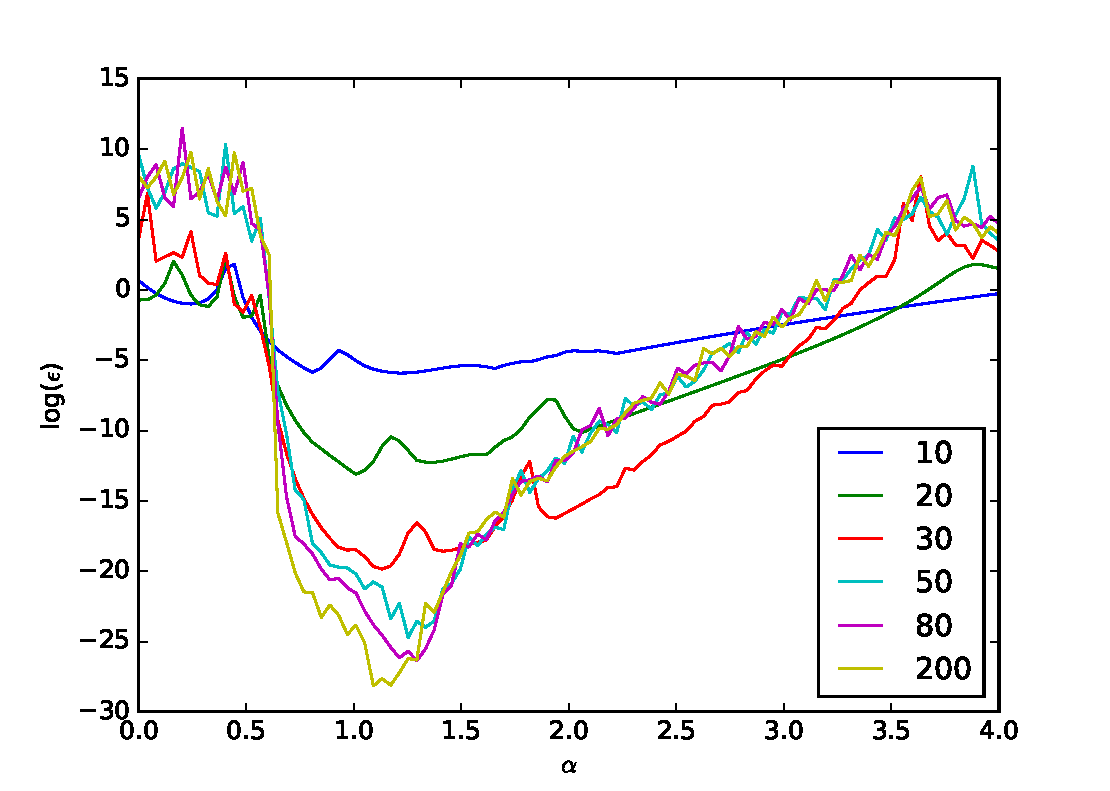
\includegraphics[width=\linewidth]{krtofl/error_phys.pdf}
\caption[LOPF: The $log$-mismatch $\epsilon$ as a function of $\alpha$]{The $log$-mismatch $\epsilon$ as a function of $\alpha$, i.e. $\epsilon(\mathfrak{v}(S_d,\alpha S_g))$. $\alpha$ scales a physical solution, i.e. when $\alpha = 1$ the corresponding $\epsilon$ is small. The number of HELM iterations $n$ is color coded.}
\label{fig:errors}
\end{figure}

In order to overcome this problem, we propose to optimize a proxy of the actual mismatch function $\epsilon$. Note that an indicator of whether or not a solution is physical is whether or not the power series coefficients $c_i[n]$ have converged to 0. Let $\bar{c}[n]$ be the mean $n$th power series coefficient of all voltages, i.e. $\bar{c}[n] = \sum_i c_i[n]/N$. Figure \ref{fig:ceps} shows a scatter-plot of $\log \bar{c}[n]$ and $\log \epsilon$. Empirically, one can see that small $\bar{c}[n]$ is a sufficient condition for small $\epsilon$, however not a necessary condition. That is, a small $\bar{c}[n]$ implies small $\epsilon$ but not vice versa. Thus in order to enforce physicality, $\bar{c}[n]$ can be minimized as a proxy for $ \epsilon$. However, one might think that optimizing $\log \bar{c}[n]$ is unnecessarily restrictive, i.e. it excludes solutions where the power series coefficients did not converge to 0 but the corresponding $v$ nevertheless fulfill the power flow equations. But, as we will show later, imposing voltage magnitude constraints naturally enforces physicality and that minimizing $\log \bar{c}[n]$ is only required after the actor function was first initialized in order to nudge the actor into the physical regime.


\begin{figure}
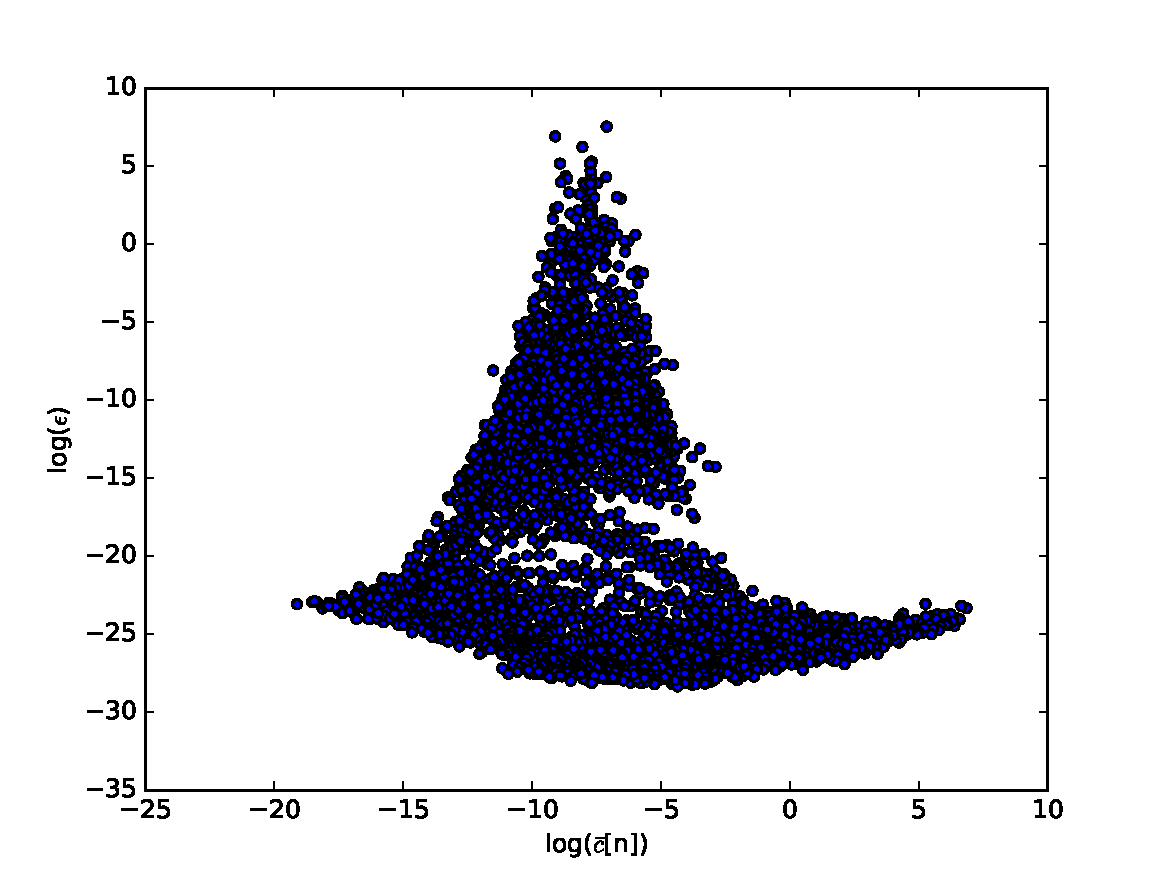
\includegraphics[width=\linewidth]{krtofl/ceps.pdf}
\caption[LOPF: Small power series coeffients imply small error.]{Small $\log \bar{c}[n]$ is a sufficient condition for small $\log(\epsilon)$. Specifically, when $\log \bar{c}[n] > -15$ then $-20 < \log(\epsilon) < -25$. However, the opposite is not true, i.e. small $\log(\epsilon)$ does not bound $\log \bar{c}[n]$.}
\label{fig:ceps}
\end{figure}

\section{Binary Constraints}
\label{sec:bin_contraints}
Binary constraints naturally occur in optimal power flow when incorporating the possibility of completely shutting down generators. Introducing this constraint make generation limit constraints non-convex, i.e. $0$ becomes a possible generation assignment, even though points between $0$ and $P^{min}$ are not valid. Typically, optimal power flow solvers employ mixed integer programming techniques such as \emph{branch and bound} or \emph{branch and cut}~\cite{lawler1966branch} algorithms to tackle this problem. However, these algorithms can incur substantial computational cost, i.e. every branch requires solving an LP relaxed optimal power flow problem and there are exponentially-many branches in a worst-case scenario.

However, using the problem formulation introduced here, because the constraint is \emph{a priori} and can be enforced by construction, we can reduce the non-convex constraint into the problem of inferring the mode of a probability distribution $P$ over binary configurations. As we will show later, because inference in $P$ is intractable, we optimize a variational bound, i.e. we introduce a variational distribution $Q_\phi$ for which posterior inference is tractable and choose the variational parameters $\phi$ in such a way that $Q_\phi$ best approximates $P$. Specifically, we built on recent advances in Bayesian inference, specifically Variational Inference~\cite{wainwright2008graphical} and train a variational distribution $Q_\phi$ parameterized by a neural network. See \cite{blei2017variational,zhang2017advances} for recent reviews of Variational Inference.

We begin by showing that computing the optimal binary configuration is equivalent to computing the mode of a distribution $P$. Let $p(b,S_d)$ be an exponential distribution and $p(b|S_d)$ its posterior (Boltzmann distribution) and $L$ be the loss as defined in (\ref{minimal_loss}), i.e. 
%\begin{align}
%p(S_g,b|S_d) = \lambda \exp(-\lambda L(b))
%\end{align}
%Note that the posterior of (22) is a Boltzmann distribution, i.e. let $B = [0,1]^N$ be the set of all possible binary configurations, then:
\begin{align}
p(b, S_d) &= \lambda \exp{- \lambda L(b\cdot S_d)}\\
p(b|S_d) &= \frac {\exp{- \lambda L(b\cdot S_d)}}{\sum _{b' \in B}{\exp{- \lambda L(b'\cdot S_d)}}} \label{p_dist}
\end{align}
It is easy to see that computing the mode of (\ref{p_dist}), i.e. $\arg\max_b p(b|S_d)$ is equivalent to choosing the binary configuration that results in the smallest loss. However, na\"ive evaluation of the mode is usually intractable, because of the intractable denominator. Naively computing the mode of (\ref{p_dist}) is equivalent to brute-force search, i.e. enumerating all possible latent configurations and picking the one with the smallest error. However, we can ensure fast inference by adopting ideas from Variational Inference~\cite{wainwright2008graphical}.

We introduce a variational distribution $Q_\phi$ whose posterior is tractable. Specifically, we choose $q(b|S_d)$ to be a multi-variate Bernoulli distribution and ensure tractability with ideas introduced in \cite{lange2018factornet}. Note that $Q_\phi$ is parameterized with a neural network, therefore ensuring that inference at test-time is fast. As a learning signal for the parameters of the auxiliary posterior distribution $\phi$, we choose the Evidence Lower Bound defined by:

\begin{align}
L_{BO}(\phi) &= \mathbb{E}_{q_\phi(b|S_d)} \log \frac{p(b,S_d)}{q_\phi(b|S_d)} \label{elbo}\\
&= \log p(S_d) - D_{KL}(q_\phi(b|S_d) || p(b|S_d))
\end{align}

Note that optimizing (\ref{elbo}) does not require knowledge of the intractable posterior of $P$ but nevertheless allows for minimizing a divergence measure between the true ($P$) and auxiliary posterior ($Q$). Thus, after training, in order to obtain an approximation of the mode of $P$, because $P$ and $Q$ will be maximally similar, posterior inference is performed on $Q$ instead.
However, the price for this `trick' is increased variance. It can be shown that the stochastic gradient estimators of (\ref{elbo}) w.r.t. $\phi$ is an unbiased but higher variance estimator of the KL-divergence~\cite{mnih2014neural}. In order to combat variance, an decades-old variance reduction technique is employed, namely sampling without replacement. Sampling without replacement from $Q$ is not trivial. However, there is a considerable body of preexisting work that we make us of. The sampling scheme introduced in \cite{shah2018without} with slight modifications is employed. Specifically, instead of using the Pareto sampler as the underlying sampling mechanism, a slightly slower but more accurate elimination sampler introduced in \cite{deville1998unequal} is used.

In order to obtain an approximation of the mode of the true posterior, because $Q$ allows for drawing samples efficiently, $S$-many samples are drawn from $Q$. Then, in order to approximate the mode of $P$, out of the $S$-many binary configurations sampled from $Q$, the one which results in the smallest loss is chosen. Note that the optimal configuration of generators is dependent on the binary configuration, thus $b$ should additionally be fed into the actor function $g$. Figure \ref{fig:pipe} shows a graphical depiction of the proposed data pipeline.
\begin{figure}
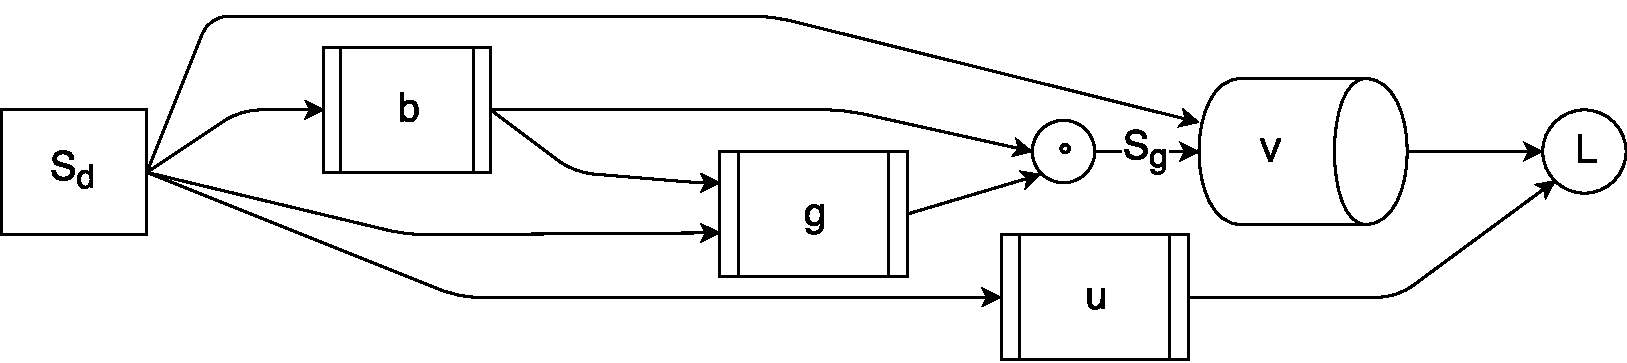
\includegraphics[width=0.95\linewidth]{krtofl/pipeline.pdf}
\caption[LOPF: Graphical depiction of the algorithmic pipeline]{A graphical depiction of the \emph{LOPF}-pipeline. Neural networks $b$ and $g$ are fed the complex demand $S_d$ and tasked with producing the optimal binary activation vector and generator configuration respectively. Because the voltages are a function of demand and generation, both are fed into the HELM based power flow solver $v$. The loss $L$ is computed based on the resulting voltages. In order to ensure that control and network inequality constraints are satisfied, a third neural network is tasked with predicting Lagrange multipliers. Because HELM is differentiable, the whole pipeline can be optimized jointly.}
\label{fig:pipe}
\end{figure}

\section{The \emph{LOPF}-algorithm}
\label{sec:LOPFalgo}
In this section we summarize the resulting algorithm, we call \emph{\textbf{L}earning \textbf{O}ptimal \textbf{P}ower \textbf{F}low}, or short \emph{LOPF}. The algorithm iterates over batches of the dataset $D$ making updates to the three constituent neural networks $g$, $b$ and $u$. For notational convenience, we define a function $solve$:
\begin{align*}
S_g &= b \cdot g_\Theta(S_d, b)\\
solve(S_d,b)
&=
\begin{pmatrix}
\epsilon(\mathfrak{v}(S_d,S_g)) \\
 c(\mathfrak{v}(S_d,S_g)) + \sum_i (u_\psi(S_d))_i k^+_i(\mathfrak{v}(S_d,S_g)) \\
N^{-1}\sum_i (f_{c,n}(S_d - S_g))_i
\end{pmatrix}^T
\end{align*}

 Below the algorithm is described in pseudo-code:


\begin{algorithm}[htb]
\SetKwInOut{Input}{input}\SetKwInOut{Output}{output}
\Input{Dataset $D$ }
\Output{Trained model parameters $\Theta, \phi$ and $\psi$}
Initialize $\Theta, \phi$ and $\psi$ randomly\;
\While{not converged}{
	\For{number of subsets of $D$}{
		select $d \subset D$\;
		\For{$S_d \in d$}{
			$\overline{G} = \{\}; G = \{\};$ \;
			$B \sim q(b|S_d)$ (without replacement)\;
			\For{$b' \in B$}{
				$\epsilon, L, c \leftarrow solve(S_d,b')$\;
				\lIf{$\epsilon < \xi$}{$G \leftarrow G \cup \{L\}$}
				\lElse{$\overline{G} \leftarrow \overline{G} \cup \{c\}$}
			}
			Compute $L_{BO}$ based on (\ref{elbo})\;
			
		}
		Maximize $L_{BO}$ w.r.t. $\phi$\;
		Maximize $\sum_{L \in G} L$ w.r.t. $\psi$\;
		Minimize $\sum_{L \in G} L$ w.r.t. $\Theta$\;
		Minimize $\sum_{c \in \overline{G}} c$ w.r.t. $\Theta$\;
	}
}
\caption{\emph{LOPF}-Algorithm in pseudo-code}
\end{algorithm}

\begin{figure}[ht]
    \centering
    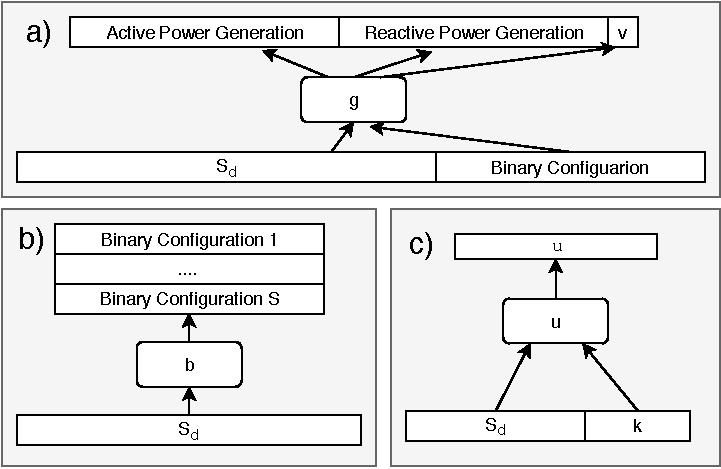
\includegraphics[width=\linewidth]{krtofl/network_structure.pdf}
    \caption[LOPF: Graphical depiction of the constituent Neural Networks.]{The input and output relationships of the three constituent neural networks. a) The actor-neural network produces active and reactive power generation for non-slack generators as well as the voltage at the slack bus given the demand $S_d$ and binary configuration produced by the $b$-network. b) The binary-network that parameterizes an auxiliary distribution. Note that the network produces multiple binary configuration by sampling from the auxiliary distribution. c) The Lagrange-network that produces a proxy of the Lagrange multipliers. Note that the constraint-violation magnitude $k$ is additionally fed into the network to ease learning.}
    \label{lopf:constituent_networks}
\end{figure}

Figure \ref{lopf:constituent_networks} shows a graphical depiction of the input/output relationships of the individual networks. Note that the actor network $g$ not only produces active and reactive generation assignments for non-slack generators but also the voltage at the slack bus. Furthermore, the magnitude by which constraints are violated, denoted by $k$, are fed into the network $u$ that produces a proxy of the Lagrange multipliers. Additionally feeding $k$ eases and speeds up learning considerably.


\section{Experiments}
\label{sec:LOPFexperiments}
Since this work introduces a learning based approach to the problem of ACOPF, the performance of the algorithm is evaluated similar to how the performance of reinforcement learning agents is evaluated, i.e. an empirical evaluation strategy is employed. Specifically, given a held out test set of load flow problems that the agent was not presented with during training, the generation cost and whether or not the agent was able to find a feasible solution are recorded. The requirements (without requirements that are met by construction) for feasibility are the following:
\begin{itemize}
    \item Log-mismatch between the RHS and LHS of the power flow equations (\ref{eq:pf_const}), i.e. $\epsilon$, must be smaller than $-10$.
    \item Slack active and reactive generation within limits
    \item Non-slack voltage magnitude constraints are met
\end{itemize}

The experiments were conducted on the 200 bus Illinois IEEE test case. However, since the IEEE test cases only contain a single demand assignment, the demand base case was superimposed by temporal patterns extracted from the RE Europe dataset \cite{re_europe}. RE Europe dataset contains historical demand and their forecasts for 3 years at an hourly interval. Let $S_{d'} \in \mathbb{C}^{200}$ be the base demand taken from test case and $x_t \in \mathbb{R}^{200 \times 26280}$ be the temporal demand patterns taken from RE Europe dataset. The temporal patterns were imposed such that the mean demand of every node is equal to the demand in the test case and such that the ratio between mean and standard deviation as seen in the RE Europe dataset is preserved. The dataset was separated into training (20.280 data points) and test set (6000) when conducting experiments.\\
The neural networks used in this experiments constitute standard fully connected three-layer networks with intermediate $tanh$ activations. All intermediate layers have $512$ hidden units.

\begin{figure*}[!ht]
    \centering
    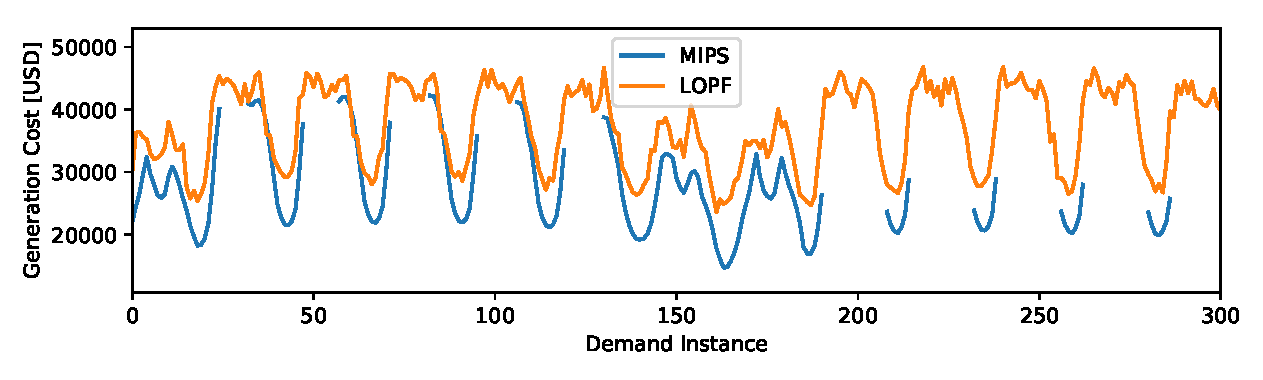
\includegraphics[width=0.85\linewidth]{krtofl/cost_comapre_uart2.pdf}
    \caption[LOPF: Comparison of generation cost.]{Comparison of generation cost on the first 300 load flow problems of the test set.}
    \label{lopf:cost}
\end{figure*}

\begin{figure*}[!ht]
    \centering
    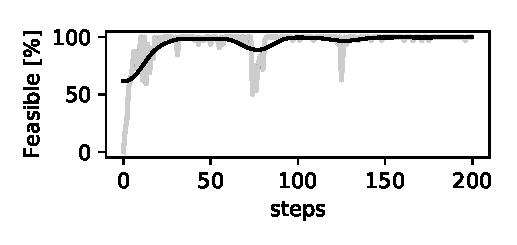
\includegraphics[width=0.48\linewidth]{krtofl/violation_percentage.pdf}
    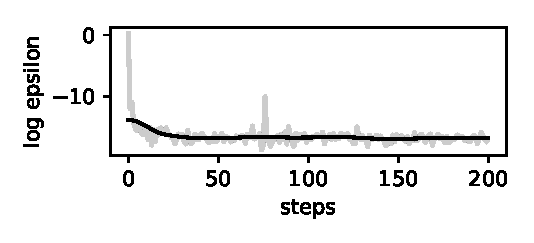
\includegraphics[width=0.48\linewidth]{krtofl/epsilon_epoch.pdf}
    \caption[LOPF: Error and feasibility as a function of learning steps.]{Left: The percentage of feasible solutions as a function of learning steps. Right: The average log mismatch of the power flow equations (\ref{eq:pf_const}) as a function of time.}
    \label{lopf:violations}
\end{figure*}

\begin{table}[]
\centering
\large
\begin{tabular}{| l | l | l |}
\hline
          & LOPF & MIPS   \\
          \hline
Feasible [\%] & 99.86  & 60.85 \\
Mean Cost [USD] & 33325.98 & 25817.55\\
Time per Instance [s] & 1.2 & 14.4\\
\hline
\end{tabular}
\caption[LOPF: Performance comparison]{Comparison of \emph{LOPF} in terms of robustness, optimality and speed on a held-out test set in comparison to MIPS.}
\label{lopf:res_table}
\end{table}

\section{Results}
\label{sec:LOPFresults}
As stated earlier, learning based approaches to control problems are usually not guaranteed to be optimal but can offer advantages in terms of computational time and robustness. The performance of \emph{LOPF} reinforces these expectations. Figure \ref{lopf:violations} (left) shows the percentage of load flow solutions produced by the agent that violate any requirement for feasibility as a function of learning steps. One learning step encompasses 32 load flow problems with 50 binary configurations each. One can see that the system quickly learns to produce feasible solutions. Initially the agent produces feasible solutions to no load flow problems. However, after just 30 steps close to all solutions proposed by the learning agent are feasible.\\
Figure \ref{lopf:violations} (right) shows the $log$-mismatch between the RHS and LHS of the power flow equations (\ref{eq:pf_const}). Note that initially, the agent produces generation assignments for which the HELM solver is unable to produce voltage phasors that fulfill the power flow equations but by minimizing the power series coefficients as described in section \ref{sec:enforcing_phys}, the agent is quickly nudged into a regime where the proposed solutions fulfill the power flow equations. However, after approximately 75 learning steps, for a short period of time, the agent produces generation assignments that, again, do not fulfill the power flow equations. This can most likely be explained by the fact that the agent also tries to minimize cost. Thus, by trying to find cheaper generation assignments, the agent left the regime in which solutions can be found by HELM but was then steered back into this regime.\\
Table \ref{lopf:res_table} showcases the performance of our proposed algorithm in comparison to the MIPS solver proposed in \cite{zimmerman2011matpower}. In order to deal with non-convex generation limit constraint, the MIPS solver was run with a unit-decommitment heuristic (\emph{runuopf}). When obtaining the results for the MIPS solver, all initializations were unchanged and only demand was varied in the way described earlier. Slightly varying the demand reveals the weakness of traditional solvers: Convergence to a feasible solution cannot be guaranteed. In our experiments, the MIPS solver produced solution which comply with all constraints and fulfill the power flow equations in only about 61\% of all problem instances (failure in 2349 out of 6000 instances). Our proposed solution produces feasible solutions for 99.86\% (failure in 8 out of 6000 cases) of the problem instances.\\
On top of that, our proposed learning agent is considerably faster than optimization based approaches: Because solutions can be obtained by feeding a demand assignment through the Neural Networks and the forward pass through Neural Nets is usually fast, obtaining the generation assignment proposed by the agent is fast. Note that when we report the time per instance for the MIPS solver, we report the mean-time over all load flow problems. However, when the solver fails, it usually fails quickly. If only the time per successful instance was reported, it would be close to 30s per instance.\\
However, Table \ref{lopf:res_table} and Figure \ref{lopf:cost} more clearly, reveal the main weakness of our proposed learning based agent. Even though solutions can be obtained robustly and fast, the proposed learning agent does not find solutions that are optimal in terms of generation cost. On average, the solutions that the agent produces are approximately 29\% more expensive than the solutions found by the MIPS solver. Note that the average cost is reported for only those load flow problems for which both approaches yielded feasible solutions.


\section{Conclusion and future work}
\label{sec:LOPFconclusion}
The main contribution of this paper is the introduction of a learning based framework for the problem of ACOPF, i.e. we translate a problem that is traditionally tackled by constrained optimization approaches into the language of learning. Specifically, we introduce a learning based approach in which an agent is tasked to produce feasible and minimal cost generation assignments as a function of the demand. A learning signal for this agent is obtained by differentiating through the operators of a load flow solver. Furthermore, we show how convex security constraints and non-convex generation limit constraint can be enforced. The resulting agent seems to produce feasible solutions fast. However, these solutions are not optimal in terms of generation cost.\\
An obvious future research path is to close the optimality gap. At this moment, because of the complexity of the resulting system, it is hard to understand why the solutions are not optimal. But note that the proposed algorithm cannot be optimal by design, because the slack generator cannot be decommitted and there is a natural interpolation between load flow solutions. However, in the opinion of the authors, performance gains in terms of optimality should be possible.\\
Another potentially interesting research question is whether or not the trained auxiliary distribution $Q$ that learns the cost surface as a function of the binary generator configuration allows for conditional sampling. Imagine a scenario where generators have failed. In such a scenario, it is paramount to reconfigure the network in a feasible state fast. If it is possible to sample from $Q$ conditioned that the failed generators are \emph{off}, then the proposed learning based agent could potentially find application in emergency situations. Note that this seemingly easy problem is not trivial because of the FactorNet~\cite{lange2018factornet} structure of the auxiliary distribution.\\
The second main contribution is the translation of the existing power flow solver HELM into the realm of \emph{optimal} power flow, specifically by showing that computing the gradients through the operations of HELM is possible. Note that this contribution is to a certain extent independent of the first contribution and in theory, any differentiable power flow solver could be plugged into the learning framework discussed above. At the same time, the findings of this work show that HELM could also be inserted into traditional optimization based approaches because its operations are differentiable. Note that when using HELM as the load flow solver for \emph{LOPF}, \emph{LOPF} is only as good as HELM. In the experience of the authors, HELM can show impressive results for some networks but then work poorly on others. An indicator for whether or not HELM will work well on a specific network is how well-behaved the `trivial' solution is about which analytical continuation is performed. Numerous tricks have been proposed to improve HELM to alleviate this problem but more research that addresses these issues might be required. Furthermore, HELM struggles with big admittance matrices.  Even though admittance matrices are usually non-singular, solving large admittance matrices as required for HELM oftentimes leads to numerical issues because they oftentimes become numerically singular. This problem could, in principle, be overcome by introducing a regularization term that vanishes when performing analytical continuation, i.e. by substituting $Y$ with $Y + (1-z)I$ with $I$ being the identity matrix. Note that this `trick' will not change the admittance matrix because at $z=1$, the regularization term will vanish.


